\subsection{Predição de enlaces em redes}

\subsubsection{Descrição do problema e hipóteses probabilísticas}

Redes sociais podem ser representadas por grafos em que cada nó é um usuário e cada
aresta indica uma relação. Um problema recorrente é prever arestas que existem mas
não foram observadas, usando apenas a estrutura conhecida do grafo. O objetivo deste
estudo é avaliar dois escores simples de predição de enlaces sobre uma rede gerada
artificialmente, medindo o quanto a estrutura observada ajuda a recuperar as arestas
ocultas.

A rede é gerada por um modelo de blocos estocásticos, no qual cada nó pertence a um
grupo e a probabilidade de aresta entre dois nós depende apenas dos grupos a que eles
pertencem. A hipótese central é que a presença de cada aresta é uma variável de
Bernoulli independente, com probabilidade dada pela Equação~\ref{eq:sbm}, em que
$p_{\text{in}}$ vale para pares do mesmo grupo e $p_{\text{out}}$ para pares de grupos
distintos \cite{chan2021probability}. Essa independência condicional aos grupos é o
que confere poder preditivo aos escores de vizinhança, pois nós de um mesmo grupo
tendem a compartilhar muitos vizinhos.

\begin{equation}
	P(A_{ij} = 1) =
	\begin{cases}
		p_{\text{in}}, & \text{se } i \text{ e } j \text{ estão no mesmo grupo} \\
		p_{\text{out}}, & \text{caso contrário}
	\end{cases}
	\label{eq:sbm}
\end{equation}

\subsubsection{Modelagem probabilística}

Foram considerados dois escores para ordenar os pares de nós sem aresta observada. O
primeiro é o número de vizinhos comuns, que conta quantos nós são simultaneamente
vizinhos de $i$ e de $j$. O segundo é o coeficiente de Jaccard da
Equação~\ref{eq:jaccard}, que normaliza os vizinhos comuns pelo total de vizinhos
distintos dos dois nós, reduzindo o efeito de nós muito conectados.

\begin{equation}
	J(i, j) = \frac{|N(i) \cap N(j)|}{|N(i) \cup N(j)|}
	\label{eq:jaccard}
\end{equation}

A qualidade de cada escore foi avaliada pela área sob a curva ROC, que mede a
probabilidade de um par realmente conectado receber escore maior que um par não
conectado. Um valor de $0{,}5$ corresponde a uma ordenação aleatória e valores
maiores indicam capacidade de predição.

\subsubsection{Implementação em R}

A rede completa tem $80$ nós divididos em dois grupos de $40$, com
$p_{\text{in}} = 0{,}25$ e $p_{\text{out}} = 0{,}05$. Após a geração, $20\%$ das
arestas existentes foram ocultadas para formar o conjunto de teste, e os escores
foram calculados para todos os pares não observados. O número de vizinhos comuns de
todos os pares é obtido de uma vez pelo produto da matriz de adjacência por ela
mesma, conforme o Listing~\ref{lst:enlace_gera}.

\begin{lstlisting}[caption={Geração da rede, ocultação de arestas e cálculo dos escores.}, label={lst:enlace_gera}]
prob_aresta <- ifelse(outer(grupo, grupo, "=="), p_in, p_out)
adj_full <- matrix(0, n, n)
ind <- lower.tri(adj_full)
adj_full[ind] <- rbinom(sum(ind), 1, prob_aresta[ind])
adj_full <- adj_full + t(adj_full)

viz_comuns <- adj_obs %*% adj_obs
grau <- rowSums(adj_obs)
\end{lstlisting}

\subsubsection{Resultados e interpretação}

Os dois escores tiveram desempenho semelhante, com área sob a curva ROC de $0{,}614$
para os vizinhos comuns e $0{,}613$ para o coeficiente de Jaccard. Ambos ficam
claramente acima de $0{,}5$, o que mostra que a estrutura observada carrega
informação útil sobre as arestas ocultas. A Figura~\ref{fig:enlaces_roc} apresenta as
curvas ROC dos dois escores frente à linha de referência da ordenação aleatória.

\begin{figure}[H]
	\centering
	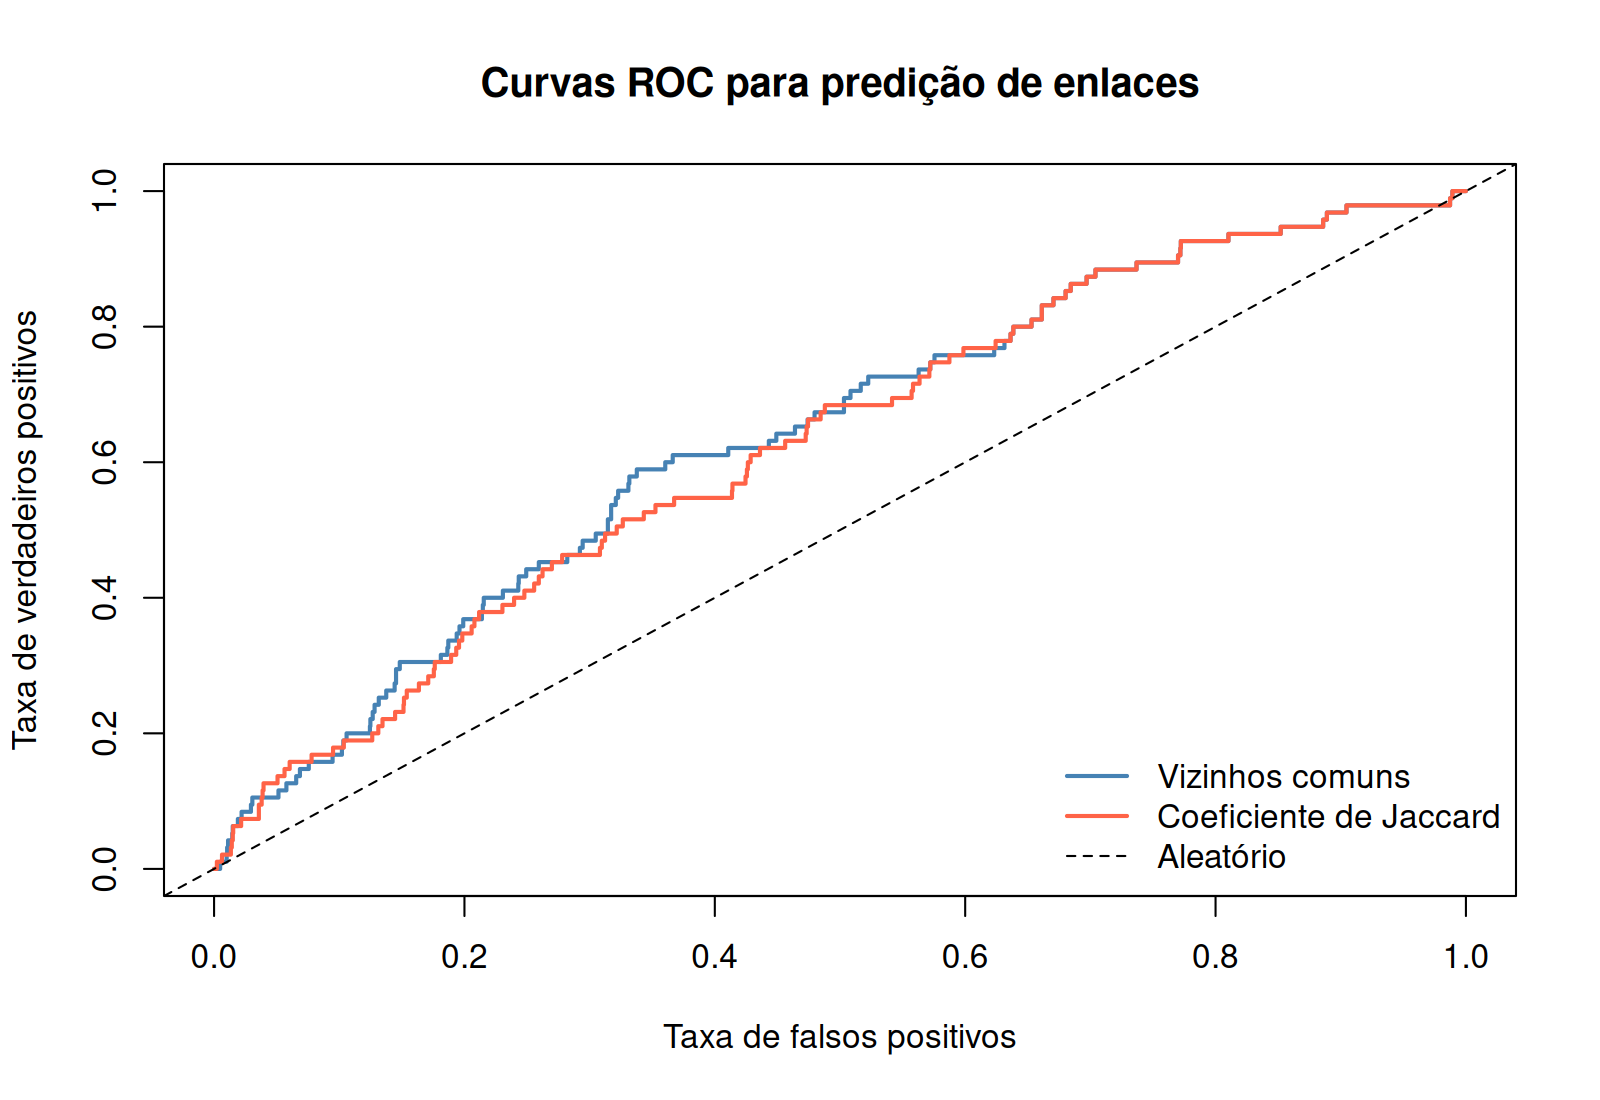
\includegraphics[width=0.8\textwidth]{secoes/07_atividade_integradora/atv_5/imagens/fig_enlaces_roc.png}
	\caption{Curvas ROC dos escores de vizinhos comuns e coeficiente de Jaccard.}
	\label{fig:enlaces_roc}
\end{figure}

A área sob a curva fica longe de $1$ porque a predição de enlaces é inerentemente
ruidosa, já que mesmo dentro de um grupo nem todos os pares estão conectados. Ainda
assim, escores baseados apenas em vizinhança recuperam parte das arestas ocultas sem
conhecer os grupos verdadeiros, o que demonstra o valor da informação estrutural. A
independência das arestas no modelo de blocos estocásticos é a hipótese que torna
essa recuperação possível, pois liga a probabilidade de uma aresta à semelhança de
vizinhança entre os nós.
